\thispagestyle{cackithitoannone}
\pagestyle{cackithitoan}
\everymath{\color{cackithi}}
\graphicspath{{../cackithi/pic/}}
%\blfootnote{{\color[named]{cackithi}$^1$Trường Đại học Mỏ--Địa chất.}}
\begingroup
\AddToShipoutPicture*{\put(0,616){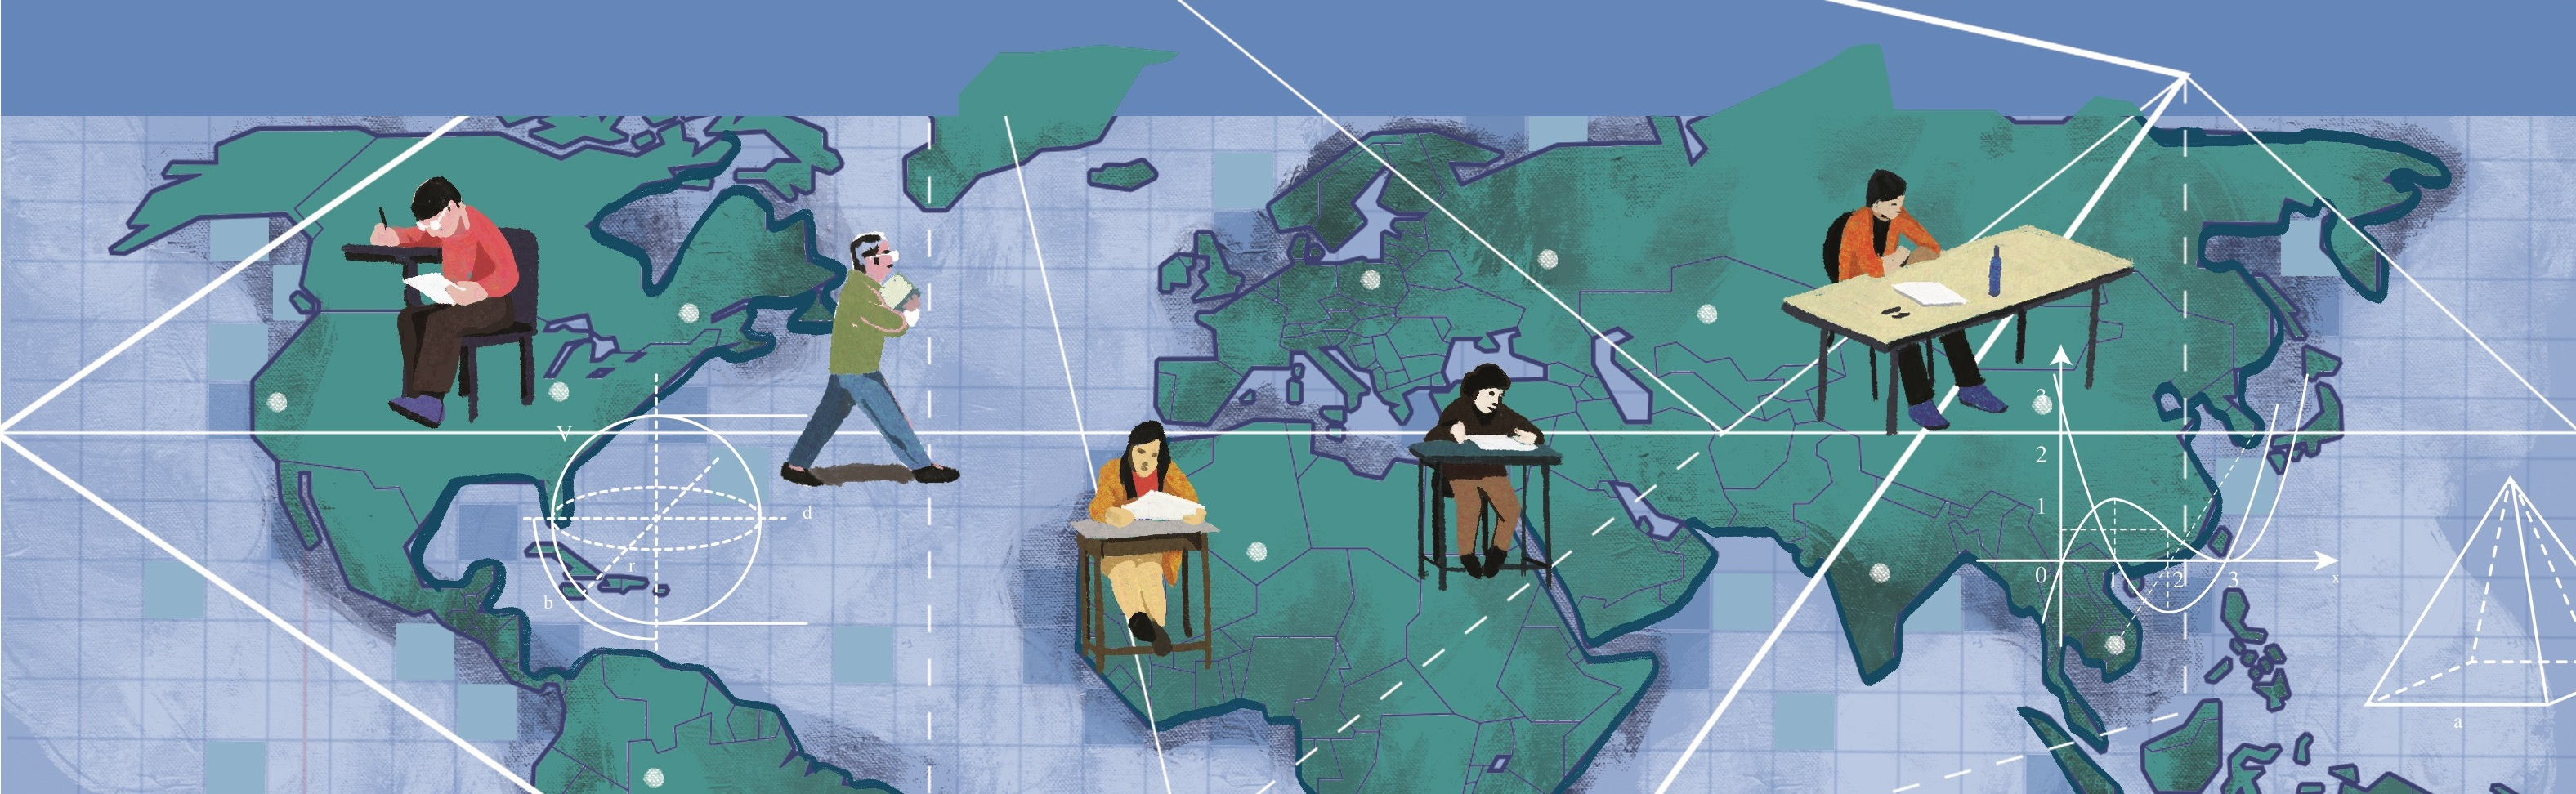
\includegraphics[width=19.3cm]{../bannercackithi}}} 
\AddToShipoutPicture*{\put(150,575){
\includegraphics[scale=1]{../tieude1.pdf}}}
\centering
\endgroup
\vspace*{130pt}

\begin{multicols}{2}
	Trong phần đầu chuyên mục, chúng tôi sẽ trình bày lời giải của các bài toán trong kỳ thi Olympic Toán thành phố Kiev (Ukraina), năm $2022$,   đăng trong số báo $8/2022$. 
	\vskip 0.1cm
	{\bf\color{cackithi} OC$\pmb{19.}$}  Viết phân số $\dfrac{1}{2021}$ thành hiệu của hai phân số tối giản có mẫu số nhỏ hơn.
	\vskip 0.1cm
	\textit{Lời giải.} Chú ý rằng $2021$ là tích của hai số nguyên tố: $2021=43\times 47$.
	\vskip 0.1cm
	Ta cần tìm $a, b$ để $\dfrac{a}{43} - \dfrac{b}{47}= \dfrac{1}{2021}$. Điều này tương đương với $47a-43b=1$. Như vậy $47a\equiv 1 \pmod{43}$, hay $4a\equiv 1\pmod{43}$. Dễ thấy ngay rằng giá trị $a=11$ thỏa mãn. Giá trị tương ứng của $b$ là $12$. Ta có 
	\begin{align*}
		\dfrac{11}{43} - \dfrac{12}{47}= \dfrac{1}{2021}.
	\end{align*} 
	Bằng cách tương tự ta cũng tìm được một cách viết khác 
	\begin{align*}
		\dfrac{35}{47} - \dfrac{32}{43}= \dfrac{1}{2021}.
	\end{align*}
	{\bf\color{cackithi} OC$\pmb{20.}$} Có $n$ tấm thẻ, trên đó viết lần lượt các số thực (không nhất thiết phân biệt): $a_1, a_2, \ldots, a_n $.  Xét tất cả $ 2^n-1 $ cách chọn ra một tập khác rỗng các tấm thẻ và tính tổng các số trên mỗi tập thẻ đã chọn. Hỏi trong số $2^n-1$ tổng nhận được có thể có nhiều nhất bao nhiêu số bằng $1$?
	\vskip 0.1cm
	Ví dụ: với $3$ tấm thẻ có số $-1$, $2$, $2$, thì các tổng thu được là $4$, $3$, $2$, $2$, $1$, $1$, $-1$. Do đó có hai tổng bằng $1$.
	\vskip 0.1cm
	\textit{Lời giải.} Trường hợp cả $n$ số trên thẻ đều bằng $0$ thì không có tổng nào bẳng $1$. Ta chỉ cần xét trường hợp có một số, giả sử là $a_1$ khác $0$. Ta có thể chia tất cả $2^n$ tập con của tập $n$ tấm thẻ thành $2^{n-1}$ cặp bằng cách ghép một tập $A$ không chứa thẻ $a_1$ với tập $A\cup \{\ \text{thẻ chứa}\ a_1\}$. Do trong mỗi cặp hai tổng nhận được có chênh lệch bằng $a_1$ nên chỉ có nhiều nhất một tập có tổng bằng $1$ (quy ước tập rỗng có tổng bằng $0$).
	\vskip 0.1cm
	Như vậy trong mọi trường hợp đều có không quá $2^{n-1}$ tổng bằng $1$. Ta dễ dàng chỉ ra ví dụ có đúng $2^{n-1}$ tổng bằng $1$:  có  $1$ tấm thẻ ghi số $1$, các tấm thẻ khác đều ghi số $0$. Như vậy có thể có nhiều nhất là $2^{n-1}$ tổng bằng $1$.
	\vskip 0.1cm
	{\bf\color{cackithi} OC$\pmb{21.}$} Trong tam giác $ ABC$, đường trung tuyến $BM$ bằng một nửa cạnh $BC$. Chứng minh rằng $ \angle ABM = \angle BCA + \angle BAC$.
	\vskip 0.1cm
	\textit{Lời giải.}
	\begin{center}
		\definecolor{qqwuqq}{rgb}{0.,0.39215686274509803,0.}
		\definecolor{uuuuuu}{rgb}{0.26666666666666666,0.26666666666666666,0.26666666666666666}
		\definecolor{xdxdff}{rgb}{0.49019607843137253,0.49019607843137253,1.}
		\definecolor{ududff}{rgb}{0.30196078431372547,0.30196078431372547,1.}
		\begin{tikzpicture}[cackithi,node font= small,scale=0.9]
			\draw [shift={(3.,0.)},color=qqwuqq] (0,0) -- (116.56505117707799:0.5) arc (116.56505117707799:180.:0.5) -- cycle;
			\draw [shift={(2.,2.)},color=qqwuqq] (0,0) -- (-63.43494882292201:0.5) arc (-63.43494882292201:0.:0.5) -- cycle;
			\draw [shift={(4.,2.)},color=qqwuqq] (0,0) -- (180.:0.5) arc (180.:243.43494882292202:0.5) -- cycle;
			\draw [shift={(-1.,0.)},color=qqwuqq] (0,0) -- (0.:0.6) arc (0.:33.690067525979785:0.6) -- cycle;
			\draw [shift={(2.,2.)},color=qqwuqq] (0,0) -- (0.:0.6) arc (0.:33.690067525979785:0.6) -- cycle;
			\draw  (4.,2.)-- (2.,2.);
			\draw  (2.,2.)-- (3.,0.);
			\draw  (2.5849705831449925,1.0983869910099906) -- (2.370308057305012,0.9910557280900002);
			\draw  (2.6296919426949894,1.0089442719099997) -- (2.4150294168550084,0.9016130089900094);
			\draw  (-1.,0.)-- (3.,0.);
			\draw  (-1.,0.)-- (5.,4.);
			\draw  (5.,4.)-- (4.,2.);
			\draw  (4.62969194269499,2.991055728090001) -- (4.415029416855009,3.0983869910099915);
			\draw  (4.584970583144993,2.901613008990009) -- (4.370308057305012,3.0089442719099995);
			\draw  (4.,2.)-- (3.,0.);
			\draw  (3.6296919426949894,0.9910557280900002) -- (3.4150294168550084,1.0983869910099906);
			\draw  (3.584970583144993,0.9016130089900094) -- (3.370308057305012,1.0089442719099997);
			\draw [shift={(-1.,0.)},color=qqwuqq] (0.:0.6) arc (0.:33.690067525979785:0.6);
			\draw[color=qqwuqq] (-0.49752668609324713,0.15213667806142553) -- (-0.35396288211988924,0.1956043003646903);
			\draw [shift={(2.,2.)},color=qqwuqq] (0.:0.6) arc (0.:33.690067525979785:0.6);
			\draw[color=qqwuqq] (2.5024733139067536,2.1521366780614257) -- (2.646037117880111,2.1956043003646903);
				\draw [fill=white] (5.,4.) circle (1.5pt);
				\draw[color=ududff] (5.2,4.33) node {$C$};
				\draw [fill=white] (3.,0.) circle (1.5pt);
				\draw[color=xdxdff] (3.2,-0.31) node {$B$};
				\draw [fill=white] (4.,2.) circle (1.5pt);
				\draw[color=uuuuuu] (4.28,1.97) node {$N$};
				\draw [fill=white] (2.,2.) circle (1.5pt);
				\draw[color=ududff] (1.7,2.35) node {$M$};
				\draw [fill=white] (-1.,0.) circle (1.5pt);
				\draw[color=uuuuuu] (-1.2,-0.23) node {$A$};
		\end{tikzpicture}
	\end{center}
	Gọi $N$ là trung điểm $BC$, ta nối đường trung bình $MN$. Khi đó ta có hai góc so le trong bằng nhau:
	\begin{align*}
		\angle ABM = \angle BMN. \tag{$1$}
	\end{align*}	
	Từ giả thiết ta có $BM= BN$ nên tam giác $BMN$ cân tại $B$.
	\vskip 0.1cm
	Như vậy $\angle BMN =\angle BNM$. \hfill ($2$)
	\vskip 0.1cm
	Từ ($1$) và ($2$) ta nhận được
	\begin{align*}
		\angle ABM= \angle BNM. \tag{$3$}
	\end{align*}
	Mặt khác ta cũng có hai góc đồng vị bằng nhau: $\angle BAC=\angle NMC$. Do đó 
	\begin{align*}
		\angle BNM&= \angle NCM + \angle NMC\\
		&= \angle BCA + \angle BAC. \tag{$4$}
	\end{align*}
	Từ ($3$) và ($4$) ta có đẳng thức cần chứng minh.
	\vskip 0.1cm
	Trong phần cuối của chuyên mục kỳ này, chúng tôi sẽ giới thiệu với bạn đọc các bài toán trong kỳ thi Olympic Toán học vùng Cáp--ca năm $2022$ (Caucasus Math Olympiad). Các bài toán này phù hợp với trình độ học sinh lớp $8-9$.
	\vskip 0.1cm
	{\bf\color{cackithi} OC$\pmb{28.}$} Cho trước các số nguyên dương $a$, $b$, $c$. Biết rằng $\dfrac{c}{b} = \dfrac{b}{a}$, và $b^2 - a - c + 1$ là số nguyên tố. Chứng minh rằng $\dfrac{a}{2}$ và $\dfrac{c}{2}$ là các số chính phương.
	\vskip 0.1cm
	{\bf\color{cackithi} OC$\pmb{29.}$} Cho hình bình hành $ABCD$, các điểm $E$ và $F$ lần lượt nằm trên các đoạn $AD$ và $CD$ sao cho $\angle BCE = \angle BAF.$ Các điểm $K$ và $L$ lần lượt nằm trên các đoạn $AD$ và $CD$ sao cho $AK = ED$ và $CL = FD$. Chứng minh rằng $\angle BKD = \angle BLD$.
	\vskip 0.1cm
	{\bf\color{cackithi} OC$\pmb{30.}$} Peter viết ra $21$ số nguyên dương đôi một phân biệt, mỗi số không lớn hơn $10^6$. Đối với mỗi cặp số $(a, b)$ được Peter viết ra, Nick  viết  số
	\begin{align*}
		F(a, b) = a + b - \gcd (a, b)
	\end{align*}
	trên mảnh giấy của mình (ở đây $\gcd$ ký hiệu ước chung lớn nhất). 
	\vskip 0.1cm
	Chứng minh rằng một trong những số mà Nick viết khác với tất cả những số mà Peter viết. 
\end{multicols}
\vspace*{-10pt}
{\color{cackithi}\rule{1\linewidth}{0.1pt}}
\vskip 0.3cm
\centerline{\LARGE{\textbf{\color{cackithi}LỜI GIẢI, ĐÁP ÁN}}}
\begin{multicols}{2}
	\textbf{\color{cackithi}Đố vui}
	\vskip 0.1cm
	Khối pho mát $1\times1\times1$ ở giữa có tất cả sáu mặt và mỗi mặt phải được tạo ra từ một lần cắt nào đó. Hơn nữa, chú ý rằng không thể dùng một lần cắt để làm lộ ra hai hay nhiều hơn những mặt này. Vì vậy, cần ít nhất $6$ lần cắt. Cuối cùng, với  $6$ lần cắt, ta có thể tạo ra $27$ miếng pho mát như yêu cầu bằng cách cắt song song với các mặt của khối lập phương. 
	\begin{figure}[H]
		\vspace*{-5pt}
		\centering
		\captionsetup{labelformat= empty, justification=centering}
		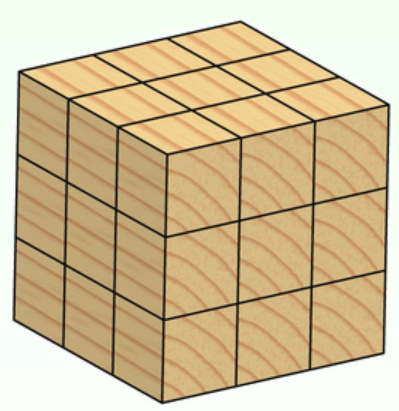
\includegraphics[width= 0.4\linewidth]{1}
		\vspace*{-10pt}
	\end{figure}
	Đáp số: $6$ lần cắt.
	\vskip 0.1cm
	\textbf{\color{cackithi}Hòn đảo kỳ lạ}
	\vskip 0.1cm 
	Xuân Phong luôn có cách để biết chính xác tuổi của mỗi người ngồi xung quanh bàn, từ đó biết được người ngồi cạnh anh ta nói thật (đến từ tộc Tutu) hay nói dối (đến từ tộc Titi). Cách xác định tuổi như sau.
	\vskip 0.1cm
	Ta chọn ra người dân cần xác định tuổi. Đặt tên anh ta, giả sử là Toto. Ta sẽ gán cho mỗi người ngồi xung quanh bàn một trong hai màu: xanh và đỏ (một cách tưởng tượng) như sau: bắt đầu gán cho Toto màu đỏ, sau đó cứ cách một người ta lại gán cho màu đỏ, những người còn lại gán cho màu xanh. Như vậy các màu xanh đỏ được ngồi xen kẽ quanh bàn, còn bản thân Toto được gán màu đỏ. 
	\vskip 0.1cm
	\hfill (Xem tiếp trang $25$.)
\end{multicols}